\paragraph{Lavpass} \mbox{} \\
Husk at reaktansen $X_C$ er avhengig av frekvens.
$$X_C = \frac{1}{2\pi f C}$$
Det tilsier at reaktansmotstanden blir lavere med høy frekvens.
\\\\
La oss se hva dette gjør med spenningen
over kondensatoren i en RC-krets.
\\
\begin{circuitikz} \draw
(0,0) to[vsourcesin, label=$Vs$] (0,2)
      to[R, label=$R$] (4,2)
      to[C, label=$X_C$] (4,0)
      -- (0,0)
(4,2) to[short, -o] (5,2)
(4,0) to[short, -o] (5,0)
      ;
\end{circuitikz}
\\
Spenningsdeling (husk: 90 grader forskyvning) for $X_C$ gir oss
$$V_{ut} = \frac{X_C}{\sqrt{X_C^2 + R^2}} \cdot V_S$$
Dette viser at spenningen ut blir lavere ved høy frekvens.
\\
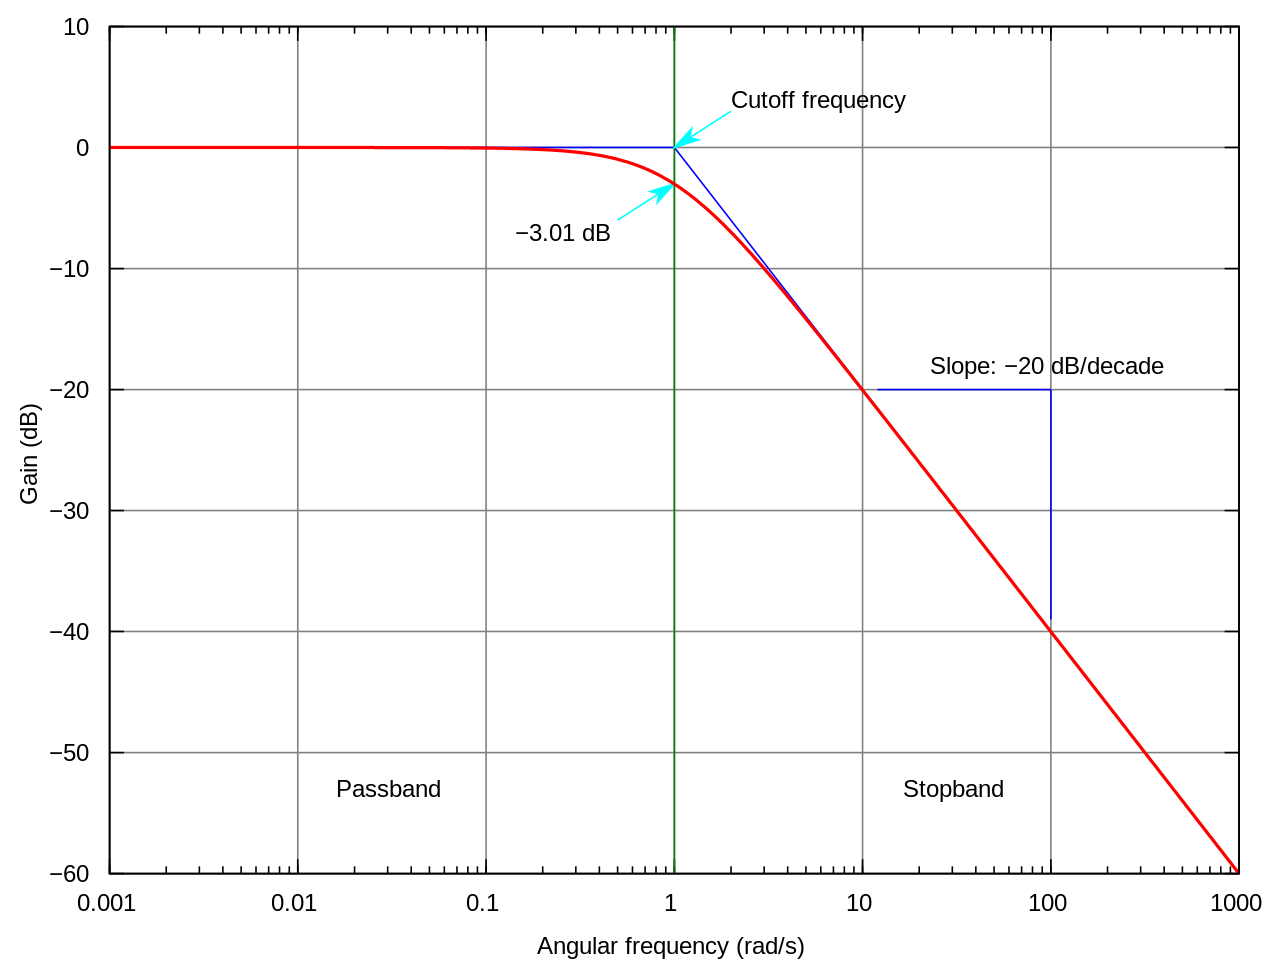
\includegraphics[width=\textwidth]{./img/lowpass}
\\
Cutoff (grense) frekvensen får man når $X_C = R$.
$$f_g = \frac{1}{2\pi R C}$$



\paragraph{Høypass} \mbox{} \\
I motsetning til et lavpassfilter som slipper gjennom lave frekvenser,
slipper høypassfiltre gjennom høye frekvenser.
\\
Dette gjøres ved å måle spenning over motstanden istedenfor kondensatoren.
\\
\begin{circuitikz} \draw
(0,0) to[vsourcesin, label=$Vs$] (0,2)
      to[C, label=$X_C$] (4,2)
      to[R, label=$R$] (4,0)
      -- (0,0)
(4,2) to[short, -o] (5,2)
(4,0) to[short, -o] (5,0)
      ;
\end{circuitikz}
\\\\
Når frekvensen blir høyere blir motstanden i kondensatoren lavere
og ved spenningsdeling blir spenningen over motstanden høyere.
\\\\
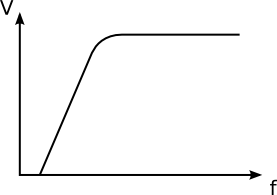
\includegraphics[width=0.5\textwidth]{./img/hpf}



\paragraph{Eksempel} \mbox{} \\
Hva er grensefrekvensen (cutoff frequency)?
\\
$R_F = \SI{100}{\ohm}$ \qquad
$C = \SI{10}{\mu \farad}$ \qquad
$R_L = \SI{910}{\ohm}$
\\
\begin{circuitikz} \draw
(0,0) node[ground]{}
      to[vsourcesin, label=$V_S$] (0,2)
      to[R, label=$R_F$] (3,2)
      to[C, label=$C$] (3,0)
      node[ground]{}
(3,2) -- (6,2)
      to[R, label=$R_L$] (6,0)
      node[ground]{}
      ;
\end{circuitikz}
\\\\
Dette kan skrives om slik vi er vant til å se thevenin
\\
\begin{circuitikz} \draw
(0,0) -- (0,4)
      -- (4,4)
      -- (4,0)
      -- (0,0)
(1,1) to[R, label=$R_F$] (1,3)
      -- (3,3)
      to[R, label=$R_L$] (3,1)
      to[vsourcesin, label=$V_S$] (1,1)
(3,3) to[short, -o] (5,3)
(3,1) to[short, -o] (5,1)
      ;
\draw[dashed]
(5,3) -- (6,3)
      to[C, label=$C$] (6,1)
      -- (5,1)
      ;
\end{circuitikz}
\\
Regner ut theveninmotstanden
$$R_{TH} = \frac{R_L \cdot R_F}{R_L + R_F} = ... = \SI{90,1}{\ohm}$$
Vi husker at cutoff frekvensen er der hvor
reaktansen og motstanden er lik.
$$X_C = R = \frac{1}{2\pi f C}$$
Løser med hensyn på f
$$f_g = \frac{1}{2\pi R C} = ... = \SI{177}{\hertz}$$
